\documentclass[a4paper, 10pt, ]{article}

\usepackage[slovak]{babel}





\usepackage[utf8]{inputenc}
\usepackage[T1]{fontenc}

\usepackage[left=4cm,
			right=4cm,
            % left=2.5cm,
			% right=5.5cm,
			top=2.1cm,
			bottom=2.6cm,
			footskip=7.5mm,
			% twoside,
			marginparwidth=3.0cm,
			%showframe,
			]{geometry}

\usepackage{graphicx}
\usepackage[dvipsnames]{xcolor}
% https://en.wikibooks.org/wiki/LaTeX/Colors


% ------------------------------

\usepackage{lmodern}

\usepackage[tt={oldstyle=false,proportional=true,monowidth}]{cfr-lm}

% ------------------------------

\usepackage{amsmath}
\usepackage{amssymb}
\usepackage{amsthm}

\usepackage{booktabs}
\usepackage{multirow}
\usepackage{array}
\usepackage{dcolumn}


\usepackage[singlelinecheck=true]{subfig}


% ------------------------------


\def\naT{\mathsf{T}}

\hyphenpenalty=6000
\tolerance=1000




% ------------------------------


\makeatletter

	\def\@seccntformat#1{\protect\makebox[0pt][r]{\csname the#1\endcsname\hspace{4mm}}}

	\def\cleardoublepage{\clearpage\if@twoside \ifodd\c@page\else
	\hbox{}
	\vspace*{\fill}
	\begin{center}
	\phantom{}
	\end{center}
	\vspace{\fill}
	\thispagestyle{empty}
	\newpage
	\if@twocolumn\hbox{}\newpage\fi\fi\fi}

	\newcommand\figcaption{\def\@captype{figure}\caption}
	\newcommand\tabcaption{\def\@captype{table}\caption}

\makeatother


% ------------------------------




\usepackage{fancyhdr}
\fancypagestyle{plain}{%
\fancyhf{} % clear all header and footer fields
\fancyfoot[C]{\sffamily {\bfseries \thepage}\ | {\scriptsize\oznacenieCasti}}
\renewcommand{\headrulewidth}{0pt}
\renewcommand{\footrulewidth}{0pt}}
\pagestyle{plain}


% ------------------------------


\usepackage{titlesec}
\titleformat{\paragraph}[hang]{\sffamily  \bfseries}{}{0pt}{}
\titlespacing*{\paragraph}{0mm}{3mm}{1mm}
\titlespacing*{\subparagraph}{0mm}{3mm}{1mm}

\titleformat*{\section}{\sffamily\Large\bfseries}
\titleformat*{\subsection}{\sffamily\large\bfseries}
\titleformat*{\subsubsection}{\sffamily\normalsize\bfseries}






% ------------------------------

\PassOptionsToPackage{hyphens}{url}
\usepackage[pdfauthor={},
			pdftitle={},
			pdfsubject={},
			pdfkeywords={},
			% hidelinks,
			colorlinks=false,
			breaklinks,
			]{hyperref}


% ------------------------------


\graphicspath{%
{../fig_standalone/}%
{../../PY/fig/}%
{../../PY/jupynotex/fig/}%
{../../ML/fig/}%
{./fig/}%
}



% ------------------------------

\usepackage{enumitem}

\usepackage{lettrine}

% ------------------------------


\usepackage{microtype}


% ------------------------------

\usepackage[titles]{tocloft}

\setlength{\cftsecindent}{-12mm}
\setlength{\cftsecnumwidth}{12mm}
\renewcommand{\cftsecpresnum}{\hfill}
\renewcommand{\cftsecaftersnum}{\hspace{4mm}}

\setlength{\cftsubsecindent}{-12mm}
\setlength{\cftsubsecnumwidth}{16mm} % 12 + 4
\renewcommand{\cftsubsecpresnum}{\hfill}
\renewcommand{\cftsubsecaftersnum}{\hspace{8mm}} % 4 + 4 mm

\setlength{\cftsubsubsecindent}{-12mm}
\setlength{\cftsubsubsecnumwidth}{20mm} % 12 + 4 + 4
\renewcommand{\cftsubsubsecpresnum}{\hfill}
\renewcommand{\cftsubsubsecaftersnum}{\hspace{12mm}} % 4 + 4 + 4 mm

\renewcommand{\cftsecpagefont}{\lstyle \bfseries}
\renewcommand{\cftsubsecpagefont}{\lstyle}
\renewcommand{\cftsubsubsecpagefont}{\lstyle}



\setlength{\cftparaindent}{-16mm}
\setlength{\cftparanumwidth}{28mm} % 16 + 4 + 4 + 4
\renewcommand{\cftparapresnum}{\hfill}
\renewcommand{\cftparaaftersnum}{\hspace{16mm}} % 4 + 4 + 4 + 4 mm








% ------------------------------

\usepackage{listings}



\renewcommand{\lstlistingname}{Výpis kódu}
\renewcommand{\lstlistlistingname}{Výpisy kódu}




%New colors defined below
\definecolor{codegreen}{rgb}{0,0.6,0}
\definecolor{codegray}{rgb}{0.5,0.5,0.5}
\definecolor{codepurple}{rgb}{0.58,0,0.82}
\definecolor{backcolour}{rgb}{0.95,0.95,0.95}

%Code listing style named "mystyle"
\lstdefinestyle{mystyle}{
  backgroundcolor=\color{backcolour},
  commentstyle=\fontfamily{lmtt}\fontsize{8.5pt}{8.75pt}\selectfont\color{codegreen},
  keywordstyle=\fontfamily{lmtt}\fontsize{8.5pt}{8.75pt}\selectfont\bfseries\color{Blue},
  stringstyle=\fontfamily{lmtt}\fontsize{8.5pt}{8.75pt}\selectfont\color{codepurple},
  basicstyle=\fontfamily{lmtt}\fontsize{8.5pt}{8.75pt}\selectfont,
  breakatwhitespace=false,
  breaklines=true,
  captionpos=t,
  keepspaces=true,
  numbers=left,
  numbersep=4mm,
  numberstyle=\fontfamily{lmtt}\fontsize{8.5pt}{8.75pt}\selectfont\color{lightgray},
  showspaces=false,
  showstringspaces=false,
  showtabs=false,
  tabsize=2,
  % xleftmargin=10pt,
  framesep=10pt,
  language=Python,
  escapechar=|,
}


\lstset{
    inputencoding=utf8,
    extendedchars=true,
    literate=%
    {á}{{\'a}}1
    {č}{{\v{c}}}1
    {ď}{{\v{d}}}1
    {é}{{\'e}}1
    {ě}{{\v{e}}}1
    {í}{{\'i}}1
    {ň}{{\v{n}}}1
    {ó}{{\'o}}1
    {ř}{{\v{r}}}1
    {š}{{\v{s}}}1
    {ť}{{\v{t}}}1
    {ú}{{\'u}}1
    {ů}{{\r{u}}}1
    {ý}{{\'y}}1
    {ž}{{\v{z}}}1
    {Á}{{\'A}}1
    {Č}{{\v{C}}}1
    {Ď}{{\v{D}}}1
    {É}{{\'E}}1
    {Ě}{{\v{E}}}1
    {Í}{{\'I}}1
    {Ň}{{\v{N}}}1
    {Ó}{{\'O}}1
    {Ř}{{\v{R}}}1
    {Š}{{\v{S}}}1
    {Ť}{{\v{T}}}1
    {Ú}{{\'U}}1
    {Ů}{{\r{U}}}1
    {Ý}{{\'Y}}1
    {Ž}{{\v{Z}}}1
    {ô}{{\^{o}}}1
}


% ------------------------------


\usepackage{caption}

\DeclareCaptionFormat{odsadene}{\protect\makebox[0pt][r]{#1#2\hspace{4mm}}#3\par}
\DeclareCaptionLabelSeparator{lendvojbodka}{:}
% \DeclareCaptionFont{lightgray}{\color{lightgray}}
\DeclareCaptionFont{lightgray}{\fontfamily{lmtt}\fontsize{8.5pt}{8.75pt}\selectfont\color{lightgray}}

\captionsetup[lstlisting]{format=odsadene, labelsep=lendvojbodka, justification=raggedright, singlelinecheck=false, labelfont={sf, lightgray},}


% ------------------------------





% ------------------------------

\usepackage[backend=biber,
            style=numeric,
            sorting=none,
            ]{biblatex}
\DeclareSourcemap{
    \maps[datatype=bibtex]{
        \map{
        \step[fieldset=note, null]
        }
        \map{
        \step[fieldset=file, null]
        }        
        % \map{
        % \step[fieldset=url, null]        
        % }
        \map{
        \step[fieldset=eprint, null]
        }
    }
}


\addbibresource{E:/_CurrentContent/01_work_repo/bibLaTeXDB/bibLaTeXDB.bib} % nonpublic data





\def\oznacenieCasti{MRS04 - ZS2023}



\usepackage{pdflscape}
\usepackage{longtable}



\begin{document}


\lstset{%
style=mystyle,
rangebeginprefix=\#\#\#\ cellB\ ,%
rangebeginsuffix=\ \#\#\#,%
rangeendprefix=\#\#\#\ cellE\ ,%
rangeendsuffix=\ \#\#\#,%
includerangemarker=false,
}




\fontsize{12pt}{22pt}\selectfont

\centerline{\textsf{Modelovanie a riadenie systémov} \hfill \textsf{\oznacenieCasti}}

\fontsize{18pt}{22pt}\selectfont





\begin{flushleft}
	\textbf{\textsf{Využitie Laplaceovej transformácie\\pri riešení diferenciálnych rovníc}}
\end{flushleft}





\normalsize

\bigskip

{\hypersetup{hidelinks}

\tableofcontents

}

\bigskip

\vspace{18pt}





\lettrine[lines=3, nindent=0pt]{K}{ využitiu} Laplaceovej transformácie pri riešení diferenciálnych rovníc patrí aj pojem \emph{prenosová funkcia}. Ak hovoríme o prenosových funkciách, hovoríme o nástroji, ktorý umožňuje analyticky pracovať s dynamickými systémami. V tomto texte však nie je cieľom priamo sa zaoberať prenosovými funkciami. Ide o širší pojem, prípadne samostaný nástroj, ktorý sa netýka len samotného riešenia diferenciálnych rovníc.


\section[Trochu o všeobecnom riešení obyčajných diferenciálnych rovníc]{Trochu o všeobecnom riešení\\obyčajných diferenciálnych rovníc}
\label{predchcasttato}


Pred tým ako budeme hovoriť o využití Laplaceovej transormácie je potrebné naznačiť isté súvislosti týkajúce sa všeobecného riešenia diferenciálnych rovníc opisujúcich dynamické systémy, také, ktoré nás tu zaujímajú. Nie je možné uvažovať akékoľvek dynamické systémy, len tie, ktoré označujeme ako lineárne a časovo invariantné. Ide o~systémy, ktoré je možné vo všeobecnosti vyjadriť obyčajnou diferenciálnou rovnicou.

Napríklad, ak by išlo o homogénnu diferenciálnu rovnicu, mala by tvar:
\begin{align} \label{vseobDifRov_h}
	\frac{\text{d}^n y(t)}{\text{d}t^n} + a_{n-1} \frac{\text{d}^{(n-1)} y(t)}{\text{d}t^{(n-1)}} + \cdots + a_0 y(t) = 0
\end{align}
kde $y(t)$ je neznáma časová funkcia (hľadáme ju ako riešenie rovnice) a, čo je značne podstatné, $a_{n-1}$ až $a_0$ sú koeficienty rovnice, reálne čísla, keďže ide o obyčajnú diferenciálnu rovnicu.

Nehomogénnou sa rovnica stáva ak uvažujeme aj iný signál ako je neznáma časová funkcia. Jednoduchý príklad by mohol byť v tvare
\begin{align} \label{vseobDifRov_nhj}
	\frac{\text{d}^n y(t)}{\text{d}t^n} + a_{n-1} \frac{\text{d}^{(n-1)} y(t)}{\text{d}t^{(n-1)}} + \cdots + a_0 y(t) = u(t)
\end{align}
kde u(t) je známa časová funkcia, z hľadiska systému predstavujúca vstup (vstupnú veličinu). Ešte všeobecnejšie zapísané:
\begin{align} \label{vseobDifRov_nh}
	\frac{\text{d}^n y(t)}{\text{d}t^n} + a_{n-1} \frac{\text{d}^{(n-1)} y(t)}{\text{d}t^{(n-1)}} + \cdots + a_0 y(t) = b_m \frac{\text{d}^m u(t)}{\text{d}t^m} + b_{m-1} \frac{\text{d}^{m-1} u(t)}{\text{d}t^{m-1}} + \cdots + b_0 u(t)
\end{align}
kde sa explicitne uvažuje aj s časovými deriváciami vstupného signálu keďže tieto jednoznačne majú súvis s dynamickým dejom ako takým. $b_{m}$ až $b_0$ sú koeficienty rovnice prislúchajúce k signálu $u(t)$ (obdobne ako $a_{xy}$ pri signále $y(t)$).


\paragraph{Linearita}

Keďže sa tu zaoberáme obyčajnými diferenciálnymi rovnicami, ktoré môžu byť vo všeobecnosti vyššieho rádu, vždy je možné takúto rovnicu zapísať ako sústavu rovníc prvého rádu. Zavádza sa pritom vektor veličín (signálov), ktoré sa označujú ako stavové veličiny. Vektor stavových veličín sa označuje $x(t)$, a výslednú sústavu diferenciálnych rovníc je možné písať v tvare
\begin{subequations} \label{LinearLTIsys}
\begin{align}
	\dot x(t) &= A x(t) + b u(t) \\
	y(t) &= c^\naT x(t)
\end{align}
\end{subequations}
kde $A$, $b$ a $c$ sú matice (vektory) zodpovedajúcich rozmerov. Pri tomto známom zápise je zrejmé, že signály systému ($x(t)$, $y(t)$, $u(t)$) a parametre systému ($A$, $b$, $c$) sú navzájom v lineárnom vzťahu. Preto sa hovorí o lineárnom dynamickom systéme.


\paragraph{Časová invariantnosť}

Navyše parametre systému ($A$, $b$, $c$) sú konštanty, nemenia sa v čase. To znamená, že vlastnosti systému sa nemenia v čase. Preto sa takýto systém označuje ako časovo invariantný.

Dôsledkom tejto vlastnosti je dôležitý fakt súvisiaci s výstupom systému ako odpoveďou na vstupný signál.

Celkovú odozvu systému na akýkoľvek vstupný signál je možné vyskladať z~postupnosti čiastkových odoziev na sériu „krátkych impulzov“ (pozri kapitolu \emph{Linear systems} v \cite{AsM08se}).

K tejto vlastnosti sa dá intuitívne dospieť ak uvažujeme vstupný signál, ktorý sa síce mení, ale pozeráme sa naň ako na signál po častiach konštantný. Takýto vstupný signál sa dá vidieť ako súčet mnohých zložiek, ktoré sa skokovo menia (každá zložka sa zmení v inom čase). Ku každej zložke možno priradiť jednoznačnú odpoveď systému a získavame tak mnoho čiastkových signálov (odpovede na jednotlivé skoky, každý v~inom čase). Označme ich $H_1(t)$, $H_2(t)$, atď. Výsledná celková odpoveď $y(t)$ je potom súčet čiastkových odpovedí $y(t) = H_1(t) + H_2(t) + \ldots$

To je možné (uvažovať) predovšetkým pre fakt, že odpoveď na skokovú zmenu na vstupe sa nemení v čase, teda je jedno, v ktorom čase nastane skok na vstupe. Kedykoľvek skok nastane, dynamická odpoveď systému je vždy rovnaká. Čiastkové odpovede $H_1(t)$, $H_2(t)$, atď. sa môžu líšiť, samozrejme, v závislosti od veľkosti skoku na vstupe. To však je prejavom statického zosilnenia systému (statických vlastností), nie dynamického deja, ktorý primárne udáva diferenciálna rovnica. Dynamiku teda možno vystihnúť napr. časovou funkciou $H(t)$, ktorá predstavuje normovanú odpoveď na skokovú zmenu vstupu (konkrétna odpoveď závisí od veľkosti skoku).

Dá sa ukázať (pozri \cite{AsM08se}), že ak budeme uvažovať o počte skokových zmien (na ktoré sú odpoveďou $H_1(t)$, $H_2(t)$, atď.) limitne sa blížiacom k nekonečnu, potom platí
\begin{align}
	y(t) = \int_0^t H^\prime(t - \tau)u(\tau) \text{d}\tau
\end{align}
kde $H^\prime(t)$ je odpoveď systému na impulz (nekonečne krátky), teda je to v princípe časová funkcia, ktorá je časovou deriváciou funkcie $H(t)$ („normovanej“ odpovede na skok).



\paragraph{Maticová exponenciálna funkcia}

Hovoríme tu o lineárnom časovo-invariantnom dynamickom systéme. Pripomeňme, že pre homogénny dynamický systém prvého rádu, teda má len jednu stavovú veličinu -- vektor $x(t)\in\mathbb R$ má len jeden prvok, je v tvare
\begin{align}
	\dot x(t) = a x(t)
\end{align}
a riešenie je
\begin{align}
	x(t) = e^{at} x(0)
\end{align}



Pre vektorový prípad (predchádzajúce je skalárny prípad), teda keď $x(t)\in\mathbb R^n$ platí, že dynamický systém je
\begin{align}
	\dot x(t) = A x(t)
\end{align}
kde $A \in\mathbb R^{n\times n}$ je matica reálnych čísiel, a riešenie je v princípe
\begin{align}
	x(t) = e^{At} x(0)
\end{align}
kde sme využili objekt $e^{At}$ čo je tzv. maticová exponenciálna funkcia. Tu sa jej definícii nebudeme venovať podrobne, čitateľa odkazujeme napr. na \cite{AsM08se}. Ide zjavne o zovšeobecnenie skalárneho prípadu (systémy prvého rádu) pre vektorový prípad (systémy vyššieho rádu). Definícia a následné využívanie matice $e^{At}$ je základom pre pojmy ako fundamentálne riešenia systému (diferenciálnej rovnice). Samotná matica $e^{At}$ sa označuje napríklad aj ako matica fundamentálnych riešení. Takpovediac „účinok“ matice $e^{At}$ je daný maticou $A$, a tú možno charakterizovať jej vlastnými číslami (a vlastnými vektormi). Tieto sú následne zdrojom definície charakteristickej rovnice (a charakteristického polynómu) tak ako sa to využíva pri hľadaní analytického riešenia diferenciálnej rovnice (ako bolo načrtnuté v predchádzajúcich učebných textoch).




\paragraph{Všeobecné riešenie homogénneho lineárneho systému}

Len pre formalizáciu uvedeného, dynamický systém bez vstupného signálu je v tvare
\begin{subequations}
\begin{align}
	\dot x(t) &= A x(t) \\
	y(t) &= c^\naT x(t)
\end{align}
\end{subequations}
a jeho riešenie, teda časová funkcia opisujúca výstup $y(t)$ je v tvare
\begin{align}
	y(t) = c^\naT e^{At} x(0)
\end{align}




\paragraph{Všeobecné riešenie nehomogénneho lineárneho systému}

V prípade, ak systém má vstupný signál $u(t)$, teda
\begin{subequations}
\begin{align}
	\dot x(t) &= A x(t) + b u(t) \\
	y(t) &= c^\naT x(t)
\end{align}
\end{subequations}
dá sa ukázať, že
\begin{align} \label{xriesLTI}
	x(t) = e^{At} x(0) + \int_0^t e^{A(t-\tau)} b u(\tau) \text{d}\tau
\end{align}
a teda samotné riešenie (výstupný signál $y(t)$) je
\begin{align}
	y(t) &= c^\naT x(t) \\
	y(t) &= c^\naT e^{At} x(0) + \int_0^t c^\naT e^{A(t-\tau)} b u(\tau) \text{d}\tau \label{riesnhrov}
\end{align}
Prvý člen (na pravej strane rovnice \eqref{riesnhrov}) sa nazýva \emph{vlastná zložka riešenia} (je vyvolaná začiatočnými podmienkami) a druhý člen sa nazýva  \emph{vnútená zložka riešenia} (je vyvolaná vstupným signálom).

\bigskip

V prvom rade si všimnime, že či už ide o odpoveď systému na začiatočnú podmienku alebo ide o odpoveď systému na vstupný signál, v oboch prípadoch je riešenie určené maticou $A$ a teda maticovou exponenciálnou funkciou $e^{At}$ vo všeobecnosti.

Druhý dôležitý moment je, že rovnica \eqref{riesnhrov} sa nazýva aj konvolučnou rovnicou, čo sa zvyčajne používa v súvislosti so špeciálnym vstupným signálom $u(t) = \delta(t)$. Signál $\delta(t)$ je známy Dirackov impulz, ide o nekonečne krátky impulz, ktorého plocha je jednotková. V týchto okolnostiach definujme
\begin{equation}
	\begin{aligned}
		h(t) &= \int_0^t c^\naT e^{A(t-\tau)} b \delta(\tau) \text{d}\tau \\
		&= c^\naT e^{At} b
	\end{aligned}
\end{equation}
čo je odpoveď systému na Dirackov impulz. To potom znamená, že celkové riešenie \eqref{riesnhrov} môžeme písať v tvare
\begin{align}
	y(t) = c^\naT e^{At} x(0) + \int_0^t h(t - \tau) u(\tau) \text{d}\tau
\end{align}

\bigskip

Za špeciálny prípad možno považovať situáciu, keď sú začiatočné podmienky nulové, vtedy
\begin{align}
	y(t) = \int_0^t h(t - \tau) u(\tau) \text{d}\tau
\end{align}
Interpretáciou uvedeného sa dostaneme k faktu, že odpoveď systému na akýkoľvek vstup $u(t)$ získame konvolúciou s časovou funkciou zodpovedajúcou impulznej odpovede systému (takzvanej impulznej charakteristiky systému).


\subsection{Pojem \emph{prenosová funkcia}}

\paragraph{Špeciálny signál $e^{st}$}


Ako sme videli v predchádzajúcom, pri riešení lineárnych dynamických systémov hrajú exponenciálne funkcie významnú úlohu. Ako dôležité sa preto črtá skúmať odpoveď systému ak vstupom je istý špeciálny signál. Ide o exponenciálny signál v tvare $e^{(\sigma + j\omega)t}$. Teda chceme skúmať vplyv špeciálneho vstupu
\begin{align}
	u(t) = e^{st}
\end{align}
kde $s = \sigma + j\omega$ (vo všeobecnosti). To, že $s$ je komplexné číslo (komplexná premenná) umožňuje považovať tento špeciálny signál vlastne za triedu signálov (rôzneho typu). Reálna časť premennej $s$ určuje exponenciálny rast alebo pokles (dokonca ak $s = 0$ potom je špeciálny signál vlastne konštantným) a imaginárna časť určuje harmonické kmitanie signálu.

Máme \eqref{xriesLTI}, a teda:
\begin{align}
	x(t) = e^{At} x(0) + \int_0^t \left( e^{A(t-\tau)} b e^{s\tau} \right) \text{d}\tau
\end{align}
kde pri manipulácii s výrazom $ \left( e^{A(t-\tau)} b e^{s\tau} \right)$ treba manipulovať s ohľadom na fakt, že ide o matice a vektory. V každom prípade, po integrácii sa získa
\begin{align}
	x(t) = e^{At} x(0) + e^{At} \left( sI - A \right)^{-1}  \left( e^{(sI-A)t} - I \right) b
\end{align}
kde $I$ je jednotková matica.

Celkové riešenie je potom
\begin{align}
	\begin{aligned}
		y(t) &= c^\naT e^{At} x(0) + c^\naT e^{At} \left( sI - A \right)^{-1}  \left( e^{(sI-A)t} - I \right) b \\
		&= c^\naT e^{At} x(0) + c^\naT e^{At} \left( sI - A \right)^{-1}  \left( e^{st} e^{-At} - I \right) b \\
		&= c^\naT e^{At} x(0) + c^\naT e^{At} \left( sI - A \right)^{-1}  \left( e^{st} e^{-At}b - b \right) \\
		&= c^\naT e^{At} x(0) +   \left(c^\naT e^{At} \left( sI - A \right)^{-1} e^{st} e^{-At}b - c^\naT e^{At} \left( sI - A \right)^{-1} b \right) \\
		&= c^\naT e^{At} x(0) +   \left(c^\naT \left( sI - A \right)^{-1} e^{st} b - c^\naT e^{At} \left( sI - A \right)^{-1} b \right)
	\end{aligned}
\end{align}
V tomto bode je možné konštatovať:
\begin{align}
	\begin{aligned}
		y(t)
		&=
		\underbrace{
		c^\naT e^{At} x(0)
		}_{\text{vlastná zložka}}
		+
		\underbrace{
		\left(c^\naT \left( sI - A \right)^{-1} e^{st} b - c^\naT e^{At} \left( sI - A \right)^{-1} b \right)
		}_{\text{vnútená zložka}}
	\end{aligned}
\end{align}
a zároveň:
\begin{align}
	\begin{aligned}
		y(t) &= c^\naT e^{At} \left( x(0) -  \left( sI - A \right)^{-1} b\right) +   \left(c^\naT  \left( sI - A \right)^{-1}  b e^{st} \right) \\
		&= c^\naT e^{At} \left( x(0) -  \left( sI - A \right)^{-1} b\right) +   \left(c^\naT  \left( sI - A \right)^{-1}  b  \right) e^{st}
	\end{aligned}
\end{align}
\begin{align}
	\begin{aligned}
		y(t)
		&=
		\underbrace{
		c^\naT e^{At} \left( x(0) -  \left( sI - A \right)^{-1} b\right)
		}_{\text{zložka opisujúca prechodné deje}}
		+
		\underbrace{
		\left(c^\naT  \left( sI - A \right)^{-1}  b  \right) e^{st}
		}_{\text{čisto exponenciálna zložka}}
	\end{aligned}
\end{align}


\paragraph{Prenosová funkcia}

O vplyve samotného špeciálneho signálu $e^{st}$ na celkové riešenie teda rozhoduje výraz $c^\naT  \left( sI - A \right)^{-1}  b$. Formálne sa
\begin{align}
	G(s) = c^\naT  \left( sI - A \right)^{-1}  b
\end{align}
nazýva prenosová funkcia systému.



\bigskip

Ak by sme sa na uvedené pozreli z hľadiska diferenciálnej rovnice opisujúcej lineárny dynamický systém, teda máme diferenciálnu rovnicu v tvare
\begin{align} \label{vseobDifRov_nh2}
	\frac{\text{d}^n y(t)}{\text{d}t^n} + a_{n-1} \frac{\text{d}^{(n-1)} y(t)}{\text{d}t^{(n-1)}} + \cdots + a_0 y(t) = b_m \frac{\text{d}^m u(t)}{\text{d}t^m} + b_{m-1} \frac{\text{d}^{m-1} u(t)}{\text{d}t^{m-1}} + \cdots + b_0 u(t)
\end{align}
potom ak na vstupe uvažujeme $u(t) = e^{st}$ a zároveň vieme, že riešenie systému je tiež nejaký exponenciálny signál, čo možno vo všeobecnosti vyjadriť ako $y(t) = y_0 e^{st}$ (kde $y_0$ najmä odlišuje $y(t)$ od $u(t)$). Ak $y(t)$ a $u(t)$ dosadíme do \eqref{vseobDifRov_nh2}, vidíme, že
\begin{align}
	\begin{aligned}
			     \frac{\text{d}^n y_0 e^{st}}{\text{d}t^n}
		+ a_{n-1} \frac{\text{d}^{(n-1)} y_0 e^{st}}{\text{d}t^{(n-1)}}
		+ \cdots
		+ a_0 y_0 e^{st}
		&=
		b_m \frac{\text{d}^m e^{st}}{\text{d}t^m}
		+ b_{m-1} \frac{\text{d}^{m-1} e^{st}}{\text{d}t^{m-1}}
		+ \cdots
		+ b_0 e^{st}
		\\
		y_0 e^{st} s^n
		+ a_{n-1}  y_0 e^{st} s^{(n-1)}
		+ \cdots
		+ a_0 y_0 e^{st}
		&=
		b_m  e^{st} s^m
		+ b_{m-1}  e^{st} s^{m-1}
		+ \cdots
		+ b_0 e^{st}
		\\
		\left(
			s^n
			+ a_{n-1}   s^{(n-1)}
			+ \cdots
			+ a_0
		\right)
		y_0 e^{st}
		&=
		\left(
		b_m   s^m
		+ b_{m-1}   s^{m-1}
		+ \cdots
		+ b_0
		\right)
		e^{st}
		\\
		y_0 e^{st}
		&=
		\frac{
		\left(
		b_m   s^m
		+ b_{m-1}   s^{m-1}
		+ \cdots
		+ b_0
		\right)
		}{
		\left(
			s^n
			+ a_{n-1}   s^{(n-1)}
			+ \cdots
			+ a_0
		\right)
		}
		e^{st}
	\end{aligned}
\end{align}
a teda môžeme povedať, že riešenie systému závislé od špeciálneho signálu $e^{st}$ je
\begin{align}
	y(t)
	&=
	\frac{
	\left(
	b_m   s^m
	+ b_{m-1}   s^{m-1}
	+ \cdots
	+ b_0
	\right)
	}{
	\left(
	s^n
	+ a_{n-1}   s^{(n-1)}
	+ \cdots
	+ a_0
	\right)
	}
	e^{st}
\end{align}
označme
\begin{subequations}
	\begin{align}
		B(s) &= \left( b_m   s^m + b_{m-1}   s^{m-1} + \cdots + b_0 \right) \\
		A(s) &=  \left( s^n + a_{n-1}   s^{(n-1)} + \cdots + a_0 \right)
	\end{align}
\end{subequations}
a výraz
\begin{align}
	G(s) = \frac{B(s)}{A(s)}
\end{align}
vyjadruje prenosovú funkciu systému.

























\section{O Laplaceovej transformácii}

Laplaceova transformácia umožnuje efektívne pracovať s lineárnymi dynamickými systémami. Transformuje a tým zjednodušuje operácie súvisiace s hľadaním riešenia lineárnych diferenciálnych rovníc (LDR). Predovšetkým zjednodušuje prácu s konvolučnou rovnicou (pozri predchádzajúcu časť~\ref{predchcasttato}).

\subsection{Definícia (v hrubých črtoch)}

Majme časovú funkciu $f(t)$ (s vhodnými vlastnosťami, ktoré tu nebudeme uvádzať). Laplaceova transformácia (LT) transformuje, či mapuje, túto funkciu na inú funkciu. Inú funkciu označme $F(s)$. LT je definovaná podľa vzťahu
\begin{align}
    F(s) = \int_0^\infty f(t) e^{-st}\text{d}t
\end{align}
kde $s$ je komplexná premenná (komplexné číslo).

Hovoríme, že ide o transformáciu z časovej oblasti (domény) do domény komplexnej premennej $s$. Premenná $s$ sa často nazýva aj Laplaceov operátor (súvislosti sa ukážu neskôr). Keďže $s = \sigma + j\omega$ a teda $e^{-(\sigma + j\omega)t}$ je signál obsahujúci vo všeobecnosti aj harmonickú (kmitavú) zložku, v tejto súvislosti hovoríme tiež, že pri LT ide o~transformáciu z časovej oblasti do frekvenčnej oblasti.

Výslednej transformovanej funkcii $F(s)$ sa hovorí tiež \emph{obraz} pôvodného signálu $f(t)$ (alebo Laplaceov obraz signálu).

LT je lineárna transformácia, t.j. ak by sme chceli transformovať súčet dvoch signálov (dvoch časových funkcií) $f(t) + g(t)$ ako celok, tak je to možné urobiť transformáciou signálov jednotlivo a až následne sčítať transformované funkcie $F(s) + G(s)$.

\subsection{Laplaceove obrazy signálov}

Majme signál $f(t)$. Laplaceovym obrazom (L-obrazom) tohto signálu je $F(s)$ (samozrejme v zmysle definície LT) a samotnú operáciu transformácie značíme ako
\begin{align}
    F(s)  =  \mathcal L \left\{ f(t) \right\} = \int_0^\infty f(t) e^{-st}\text{d}t
\end{align}




\subsubsection{Derivácia}

Nájdime L-obraz signálu $\frac{\text{d}f(t)}{dt}$ (alebo teda signálu $\dot f(t)$), teda
\begin{align}
    \mathcal L \left\{ \frac{\text{d}f(t)}{dt} \right\} = \int_0^\infty \frac{\text{d}f(t)}{\text{d}t} e^{-st}\text{d}t
\end{align}
Tento integrál je možné nájsť metódou per partes, pri ktorej vo všeobecnosti platí
\begin{align}
    \int_0^\infty u(t)v^\prime(t)\text{d}t = \left[ u(t)v(t) \right]_0^\infty - \int_0^\infty u^\prime(t) v(t) \text{d}t
\end{align}
Uvažujme tu $u(t) = e^{-st}$ a $v(t) = f(t)$, potom
\begin{equation}
    \begin{aligned}
        \int_0^\infty \frac{\text{d}f(t)}{\text{d}t} e^{-st}\text{d}t
            &=  \left[ e^{-st} f(t) \right]_0^\infty - (-s)  \int_0^\infty f(t) e^{-st}\text{d}t \\
            &= 0 - f(0) + s F(s) \\
            &= s F(s) - f(0)
    \end{aligned}
\end{equation}
je L-obraz signálu $\frac{\text{d}f(t)}{dt}$.



\subsubsection{Integrál}

Obdobne by sme mohli hľadať aj obraz signálu $\int_0^t f(\tau) \text{d}\tau$, teda
\begin{align}
    \mathcal L \left\{ \int_0^t f(\tau) \text{d}\tau \right\} = \int_0^\infty \left(\int_0^t f(\tau) \text{d}\tau \right) e^{-st}\text{d}t
\end{align}
Hľadajme L-obraz tak, že zavedieme signál $g(t) = \int_0^t f(\tau) \text{d}\tau$ čo potom znamená, že $\dot g(t) = f(t)$. Hľadáme $\mathcal L \left\{ g(t) \right\} = G(s)$. Najskôr si však všimnime, že
\begin{equation}
    \begin{aligned}
        \mathcal L \left\{ \dot g(t) \right\} =& s G(s) - g(0) \\
        & s G(s) - g(0) = F(s)
    \end{aligned}
\end{equation}
a k tomu vidíme, že $g(0) = \int_0^0 f(\tau) \text{d}\tau = 0$. Teda
\begin{subequations}
    \begin{align}
        sG(s) &= F(s) \\
        G(s) &= \frac{1}{s} F(s)
    \end{align}
\end{subequations}
čím sme našli
\begin{align}
    \mathcal L \left\{ \int_0^t f(\tau) \text{d}\tau \right\} = \frac{1}{s} F(s)
\end{align}



\subsubsection{Obraz Dirackovho impulzu}

Dirackov impulz je signál taký, že (napríklad)
\begin{align}
    \delta(t) =
    \left\{
        \begin{aligned}
            &0 & \text{ak $t \neq 0$} \\
            &\infty & \text{ak $t = 0$}
        \end{aligned}
    \right.
\end{align}
pričom z princípu platí
\begin{align}
    \int_{-\infty}^\infty \delta(\tau) \text{d}\tau = 1
\end{align}

Totiž, v závislosti od toho ako by sme presnejšie matematicky špecifikovali Dirackov impulz $\delta(t)$ by sa konkrétne spôsoby aplikácie LT (výpočet integrálu) mohli formálne líšiť, avšak v každom prípade vždy platí
\begin{align}
    \mathcal L \left\{ \delta(t) \right\} = 1
\end{align}


\subsubsection{Obraz jednotkového skoku}
Pri tzv. jednotkovom skoku sa uvažuje, že v čase $0$ sa hodnota signálu skokovo zmení z $0$ na $1$ (má hodnotu „jedna jednotka“). Keďže sa tu nachádzame len v čase väčšom ako nula, môžeme uvažovať, že tu hľadáme obraz signálu $f(t) = 1$, teda
\begin{equation}
    \begin{aligned}
        \mathcal L \left\{ 1 \right\} &= \int_0^\infty 1 e^{-st}\text{d}t \\
        &= \left[ - \frac{1}{s} e^{-st} \right]_0^\infty \\
        &= 0 - \frac{1}{s} e^{-s0} \\
        &= \frac{1}{s}
    \end{aligned}
\end{equation}




\subsubsection{Obraz exponencialnej funkcie}
\label{vyhlcast}

Nájdime obraz $f(t) = e^{at}$.
\begin{equation}
    \begin{aligned}
        F(s) &= \int_0^\infty e^{at} e^{-st}\text{d}t \\
        &= \int_0^\infty e^{(a-s)t}\text{d}t \\
        &= \left[ \frac{1}{a-s} e^{(a-s)t} \right]_0^\infty \\
        &= 0 - \frac{1}{a-s} \\
        &= \frac{1}{s - a}
    \end{aligned}
\end{equation}



\subsubsection{Obraz čaového posunutia}

Majme signál $f(t)$. Signál posunutý v čase je $f(t-D)$ (v zmysle vstupno-výstupného oneskorenia, alebo dopravného oneskorenia). Obrazom $f(t)$ je $F(s)$. Obrazom $f(t-D)$ je
\begin{align}
    \int_0^\infty f(t-D) e^{-st} \text{d}t
\end{align}
Zaveďme substitúciu $\tau  = t-D$, teda $t=\tau+D$ a tiež $\text{d}t = \text{d}\tau$ keďže $D$ je v čase konštantné. Potom
\begin{align}
    \int_0^\infty f(\tau) e^{-s(\tau+D)} \text{d}\tau = e^{-sD} \int_0^\infty f(\tau) e^{-s\tau} \text{d}\tau
\end{align}
a je zrejmé, že
\begin{align}
    e^{-sD} F(s)
\end{align}
je obrazom posunutého signálu $f(t-D)$.





\subsection{Laplaceov obraz riešenia homogénnej diferenciálnej rovnice}

\paragraph{Príklad}

Majme diferenciálnu rovnicu
\begin{align}  \label{prrov}
    \dot y(t) - a y(t) = 0 \quad y(0) = y_0
\end{align}
Na jednotlivé signály v tejto rovnici aplikujme LT.
\begin{align}
    \left( s Y(s) - y(0)  \right) - a Y(s) = 0
\end{align}
kde $Y(s)$ je obrazom signálu $y(t)$. $Y(s)$ je teda obrazom riešenia rovnice. Vyjadrime $Y(s)$:
\begin{align}
    \begin{aligned}
        (s-a)Y(s) - y(0) &= 0 \\
        Y(s) &= \frac{1}{(s-a)} y(0)
    \end{aligned}
\end{align}

Otázka je, ak poznáme signál v s-oblasti (v Laplaceovej doméne), vieme určiť pôvodný signál v časovej oblasti? Vieme nájsť pomocou obrazu riešenia $Y(s)$ samotné riešenie $y(t)$?

V tomto prípade je vzhľadom na časť~\ref{vyhlcast} jasné, že
\begin{align} \label{prries}
    \mathcal L ^{-1} \left\{ Y(s) \right\} = y(t) = e^{at}y(0)
\end{align}
kde $\mathcal L ^{-1} \left\{  \right\}$ predstavuje  inverznú LT transformáciu.

Tiež tu vieme, že \eqref{prries} je správne riešenie diferenciálnej rovnice \eqref{prrov}.

\subsubsection{Inverzná Laplaceova transformácia}

Značíme ju ako
\begin{align}
    \mathcal L ^{-1} \left\{ F(s) \right\} = f(t)
\end{align}
pričom formálne ide o operáciu definovanú vzťahom
\begin{align}
    f(t) = \frac{1}{2\pi j} \int_{\sigma-j\omega}^{\sigma + j\omega} F(s) e^{st} \text{d}s
\end{align}

Výpočet inverznej LT spravidla nie je jednoduchý. V praxi sa využíva tabuľka LT (pozri časť~\ref{Tabuľka Laplaceových obrazov}), ktorá uvádza L-obrazy a k nim prislúchajúce časové signály. Tabuľka obsahuje výber typických a dôležitých signálov využívaných pri analýze dynamických systémov.

Zložitý obraz riešenia diferenciálnej rovnice je zväčša možné upraviť tak, že je v~ňom vidieť jednotlivé dielčie obrazy zodpovedajúce typickým signálom (uvedeným v tabuľke LT). Z typických časových signálov sa potom vyskladá časová funkcia zodpovedajúca celkovému riešeniu (v časovej oblasti).





\subsection{Laplaceov obraz riešenia nehomogénnej diferenciálnej rovnice}

\paragraph{Príklad}

Majme rovnicu
\begin{align}
    \ddot y(t) +4 \dot y(t) + 3y(t) = u(t) \quad y(0) = 3, \dot y(0) = -2
\end{align}
kde vstupný signál $u(t) = 12$ (konštantný v čase). Aplikujme LT
\begin{align}
    \big( s \mathcal L \{\dot y\} - \dot y(0) \big) + 4 \left( sY(s) - y(0) \right) + 3 Y(s) &=  U(s) \\
    \Big( s \big( sY(s) - y(0) \big) - \dot y(0) \Big) + 4sY(s) - 4y(0) + 3Y(s) &= U(s) \\
    s^2Y(s) - sy(0) - \dot y(0)  + 4sY(s) - 4y(0) + 3Y(s) &= U(s) \\
    s^2Y(s)   + 4sY(s)  + 3Y(s) - sy(0) - \dot y(0) - 4y(0) &= U(s)
\end{align}
a teda
\begin{align}
    \left( s^2   + 4s  + 3\right)Y(s) &= sy(0) +  \dot y(0) + 4y(0) + U(s) \\
    Y(s) &= \frac{sy(0) +  \dot y(0) + 4y(0)}{\left( s^2   + 4s  + 3\right)} + \frac{1}{\left( s^2   + 4s  + 3\right)}U(s)
\end{align}

Poznáme aj konkrétny tvar obrazu $U(s)$, keďže $u(t) = 12$, tak $U(s) = 12 \frac{1}{s}$, teda
\begin{align}
    Y(s) &= \frac{sy(0) +  \dot y(0) + 4y(0)}{\left( s^2   + 4s  + 3\right)} + \frac{1}{\left( s^2   + 4s  + 3\right)} 12 \frac{1}{s}
\end{align}
a toto je obrazom riešenia diferenciálnej rovnice.

Všimnime si, že sú tu prítomné dve zložky
\begin{align} \label{vvzlozky}
    Y(s)
    &=
    \underbrace{
    \frac{3s + 10}{\left( s^2   + 4s  + 3\right)}
    }_{\text{vlastná zložka}}
    +
    \underbrace{
    \frac{12}{\left( s^2   + 4s  + 3\right) s}
    }_{\text{vnútená zložka}}
\end{align}
kde sme aj číselne dosadili hodnoty začiatočných podmienok.

Keď je obraz riešenia v tvare \eqref{vvzlozky} je prakticky nemožné priradiť k nemu originálny časový signál -- nie sú tam očividné typické obrazy typických signálov.

Rozložme na parciálne zlomky
\begin{align}
    \frac{3s + 10}{\left( s^2   + 4s  + 3\right)} &= \frac{7}{2(s+1)} - \frac{1}{2(s+3)} \label{pz1} \\
    \frac{12}{\left( s^2   + 4s  + 3\right) s} &= \frac{4}{s} - \frac{6}{(s+1)} + \frac{2}{(s+3)} \label{pz2}
\end{align}
a tým sa hneď stáva zrejmé, že \eqref{pz1} má originál
\begin{align}
    y_{vlast}(t) = \frac{7}{2} e^{-t} - \frac{1}{2} e^{-3t}
\end{align}
a \eqref{pz2} ma originál
\begin{align}
    y_{vnut}(t) = 4 - 6 e^{-t} + 2 e^{-3t}
\end{align}
Celkové riešenie je
\begin{align}
    \begin{aligned}
        y(t) &= \frac{7}{2} e^{-t} - \frac{1}{2} e^{-3t} +  4 - 6 e^{-t} + 2 e^{-3t} \\
        &= 4 - \frac{5}{2} e^{-t} + \frac{3}{2} e^{-3t}
    \end{aligned}
\end{align}



\subsubsection{Prenosové funkcie}

Ak by sme uvažovali diferenciálnu rovnicu (vo všeobecnosti, ale tu to uvedieme na konkrétnejšom prípade pre lepšie uchopenie)
\begin{align}
    \ddot y(t) + a_1 \dot y(t) + a_0 y(t) = b_1 \dot u(t) + b_0 u(t)
\end{align}
avšak pri nulových začiatočných podmienkach a to na oboch stranách, teda $\dot y(0) = 0$, $y(0) = 0$ a $u(0) = 0$, potom aplikovaním LT máme
\begin{align}
    s^2 Y(s)   + a_1 s Y(s)  + a_0 Y(s) &= b_1 s U(s) + b_0 U(s) \\
    (s^2   + a_1 s   + a_0) Y(s) &= (b_1 s  + b_0) U(s)
\end{align}
Obraz riešenia samozrejme je
\begin{align}
    Y(s) &= \frac{(b_1 s  + b_0)}{(s^2   + a_1 s   + a_0)} U(s) \\
    Y(s) &= \frac{B(s)}{A(s)} U(s)
\end{align}
kde sme pre všeobecnosť zaviedli označenie príslušných polynómov $A(s)$ a $B(s)$.

Racionálna funkcia
% $
\begin{align}
    \frac{B(s)}{A(s)}
\end{align}
% $
dáva do vzťahu vstup systému $U(s)$ (jeho obraz) s~výstupom systému $Y(s)$. Táto racionálna funkcia sa nazýva prenosová funkcia.

Inými slovami, prenosová funkcia je pomer obrazu výstupného signálu k obrazu vstupného signálu pri nulových začiatočných podmienkach.
\begin{align}
    \frac{Y(s)}{U(s)} = \frac{B(s)}{A(s)}
\end{align}
Formálne sa prenosová funkcia označuje aj ako celok:
\begin{align}
    G(s) = \frac{B(s)}{A(s)}
\end{align}




\newpage

\section{Tabuľka Laplaceových obrazov}
\label{Tabuľka Laplaceových obrazov}



% Pozri tabuľku~\ref{Laplaceove obrazy signálov}\footnote{Ak tabuľka obsahuje chyby, nie je to zámer, iba lenivosť.}




\newcommand{\Laplace}[1]{\ensuremath{\mathcal{L}{\left\{#1\right\}}}}
\newcommand{\InvLap}[1]{\ensuremath{\mathcal{L}^{-1}{\left\{#1\right\}}}}


    \begin{longtable}{cc}

        \toprule
        $f(t)$                                  & $\Laplace{f(t)}=F(s)$ \\
        \midrule
        \endhead
        \addlinespace[3mm]
        $1$                                     &    			  $\dfrac{1}{s}$                        \\ \addlinespace[3mm]
        $e^{at}f(t)$	                        & $F(s-a)$	                                            \\ \addlinespace[3mm]
        % $\mathcal{U}(t-a)$                      & $\dfrac{e^{-as}}{s}$                                  \\ \addlinespace[3mm]
        % $f(t-a)\mathcal{U}(t-a)$                & $e^{-as}F(s)$                                         \\ \addlinespace[3mm]
        $\delta(t)$	                            & $1$                                                   \\ \addlinespace[3mm]
        $\delta(t-t_0)$                         & $e^{-st_0}$                                           \\ \addlinespace[3mm]
        $t^nf(t)$ 	                            & $(-1)^n\dfrac{\text{d}^n F(s)}{\text{d} s^n}$                          \\ \addlinespace[3mm]
        $\dot f(t)$ 	                            & $sF(s) - f(0)$                                       \\ \addlinespace[3mm]
        $\displaystyle \frac{\text{d}^n f(t)}{\text{d}t^n}$ 	                            & $s^nF(s) - s^{(n-1)} f(0) - \cdots - f^{(n-1)}(0)$    \\ \addlinespace[3mm]
        $\displaystyle{\int_0^t f(x)g(t-x) \text{d}x}$  & $F(s)G(s)$                                            \\ \addlinespace[3mm]
        $t^n$ ($n=0,1,2,\dots$)                 & $\dfrac{n!}{s^{n+1}}$                                 \\ \addlinespace[3mm]
        $\sin kt$ 	                            & $\dfrac{k}{s^2+k^2}$                                   \\ \addlinespace[3mm]
        $\cos kt$ 	                            & $\dfrac{s}{s^2+k^2}$                                   \\ \addlinespace[3mm]
        $e^{at}$ 	                            & $\dfrac{1}{s-a}$ 	                                      \\ \addlinespace[3mm]
        $\sinh kt$	                            & $\dfrac{k}{s^2-k^2}$                                   \\ \addlinespace[3mm]
        $\cosh kt$	                            & $\dfrac{s}{s^2-k^2}$                                   \\ \addlinespace[3mm]
        $\dfrac{e^{at}-e^{bt}}{a-b}$	        & $\dfrac{1}{(s-a)(s-b)}$                                  \\ \addlinespace[3mm]
        $\dfrac{ae^{at}-be^{bt}}{a-b}$	        & $\dfrac{s}{(s-a)(s-b)}$                                \\ \addlinespace[3mm]
        $te^{at}$	                            & $\dfrac{1}{(s-a)^2}$	                                   \\ \addlinespace[3mm]
        $t^ne^{at}$	                            & $\dfrac{n!}{(s-a)^{n+1}}$	                                \\ \addlinespace[3mm]
        $e^{at}\sin kt$	                        & $\dfrac{k}{(s-a)^2+k^2}$                                  \\ \addlinespace[3mm]
        $e^{at}\cos kt$	                        & $\dfrac{s-a}{(s-a)^2+k^2}$                                \\ \addlinespace[3mm]
        $e^{at}\sinh kt$	                    & $\dfrac{k}{(s-a)^2-k^2}$                                 \\ \addlinespace[3mm]
        $e^{at}\cosh kt$	                    & $\dfrac{s-a}{(s-a)^2-k^2}$                               \\ \addlinespace[3mm]
        $t\sin kt$  	                        & $\dfrac{2ks}{(s^2+k^2)^2}$                               \\ \addlinespace[3mm]
        $t\cos kt$  	                        & $\dfrac{s^2-k^2}{(s^2+k^2)^2}$                           \\ \addlinespace[3mm]
        $t\sinh kt$  	                        & $\dfrac{2ks}{(s^2-k^2)^2}$                              \\ \addlinespace[3mm]
        $t\cosh kt$  	                        & $\dfrac{s^2+k^2}{(s^2-k^2)^2}$                          \\ \addlinespace[3mm]
        $\dfrac{\sin at}{t}$	                & $\arctan \dfrac{a}{s}$                                   \\ \addlinespace[3mm]
        $\dfrac{1}{\sqrt{\pi t}}e^{-a^2/4t}$	& $\dfrac{e^{-a\sqrt{s}}}{\sqrt{s}}$                           \\ \addlinespace[3mm]
        $\dfrac{a}{2\sqrt{\pi t^3}}e^{-a^2/4t}$	& $e^{-a\sqrt{s}}$                                      \\ \addlinespace[3mm]
        % $\text{erfc}\left(\dfrac{a}{2\sqrt{t}}\right)$ &  $\dfrac{e^{-a\sqrt{s}}}{s}$                       \\ \addlinespace[3mm]

        % \bottomrule

    \end{longtable}




















\section{Príklady}



\paragraph{Príklad 1}

Majme diferenciálnu rovnicu
\begin{align}
    \dot y(t) - a y(t) = u(t) \quad y(0) = 0
\end{align}
kde $a \in \mathbb R$ je parameter a $u(t) = \delta(t)$, čo je Dirackov impulz v čase $0$. Uplatnením Laplaceovej transformácie
\begin{align}
    sY(s) - y(0) - a Y(s) = U(s)
\end{align}
kde $U(s) = 1$, teda
\begin{align}
    Y(s) = \frac{1}{s - a}
\end{align}

Spätná Laplaceova transformácia potom vedie na
\begin{align}
    y(t) = e^{at}
\end{align}
čo je riešenie pôvodnej diferenciálnej rovnice.



\paragraph{Príklad 2}

Majme diferenciálnu rovnicu
\begin{align}
    \dot y(t) - a y(t) = 0 \quad y(0) = y_0
\end{align}
kde $a \in \mathbb R$ je parameter a $y_0$ je hodnota začiatočnej podmienky. Uplatnením Laplaceovej transformácie
\begin{align}
    sY(s) - y(0) - a Y(s) = 0
\end{align}
teda
\begin{align}
    Y(s) = \frac{1}{s - a} y(0)
\end{align}

Spätná Laplaceova transformácia potom vedie na
\begin{align}
    y(t) = e^{at} y(0)
\end{align}
čo je riešenie pôvodnej diferenciálnej rovnice.


\paragraph{Postreh k príkladu 1 a 2}
Riešenie systému prvého rádu (čo je len „slang“ pre riešenie diferenciálnej rovnice prvého rádu opisujúcej dynamický systém), ktorý má nulový (žiadny) vstup ale má nenulovú začiatočnú podmienku je $y(t) = e^{at} y(0)$. Riešenie systému prvého rádu, ktorý má nulovú začiatočnú podmienku ale na vstupe má Dirackov impulz (signál $\delta(t)$) je $y(t) = e^{at}$ pričom ak by sme zovšeobecnili vstup spôsobom $u(t) = y_0 \delta(t)$, teda zaviedli sme faktor $y_0$, potom riešenie je zjavne $y(t) = e^{at} y_0 $. Začiatočná podmienka $y(0)$ a faktor $y_0$ plnia tú istú úlohu. Čo znamená, že pomocou Dirackovho impulzu je možné nahradiť vplyv začiatočnej podmienky systému. Nevýhodou je, že v praxi nie je možné realizovať Dirackov impulz, keďže má nekonečne malú šírku, len jeho aproximáciu, ktorou je impulz s relatívne malou šírkou.





\paragraph{Príklad 3}

Majme diferenciálnu rovnicu
\begin{align}
    \dot y(t) - a y(t) = u(t) \quad y(0) = 0
\end{align}
kde $a \in \mathbb R$ je parameter a $u(t) = 1$. Potom
\begin{align}
    Y(s) - y(0) - aY(s) = U(s)
\end{align}
kde $U(s) = \frac{1}{s}$, teda
\begin{align}
    (s - a)Y(s) &= \frac{1}{s} \\
    Y(s) &= \frac{1}{(s-a)s}
\end{align}

Rozložme pravú stranu na parciálne zlomky, teda
\begin{align} \label{tmppredrozkladom}
    \frac{1}{(s-a)s} = \frac{K_1}{s-a} + \frac{K_2}{s}
\end{align}
kde $K_1 \in \mathbb R$ a $K_2 \in \mathbb R$ sú konštanty (reálne čísla), ktoré je potrebné nájsť. Upravme~\eqref{tmppredrozkladom}
\begin{align}
    1 = K_1 s + K_2 (s - a)
\end{align}
Vidíme, že v tomto prípade sú dve možnosti, keď $s = 0$, vtedy $K_2 = - \frac{1}{a}$, a keď $s = a$, vtedy $K_1 = \frac{1}{a}$, takže
\begin{align}
    Y(s) = \frac{\frac{1}{a}}{s-a} - \frac{\frac{1}{a}}{s}
\end{align}

Využitím tabuľky obrazov LT (v časti~\ref{Tabuľka Laplaceových obrazov}) máme
\begin{align}
    y(t) = \frac{1}{a} e^{at} - \frac{1}{a}
\end{align}
čo je riešenie pôvodnej diferenciálnej rovnice.













\paragraph{Príklad pre širší rozhľad}

Majme diferenciálnu rovnicu:
\begin{equation} \label{Zadaná rovnica}
	\dddot{y} + 5,4 \ddot{y} + 9,7 \dot{y} + 5,592 y = 2 e^{-1,2t}
\end{equation}
Zvoľme nenulové začiatočné podmienky nasledovne:
\begin{equation*}
		y(0) = 1 \qquad \dot{y}(0)  = 1 \qquad 	\ddot{y}(0) = 1
\end{equation*}

Rovnica \eqref{Zadaná rovnica} má po Laplaceovej transformácii tvar
\begin{equation}
	s^3Y - s^2 - s - 1 + 5,4 \left( s^2Y - s - 1 \right) + 9,7 \left( sY - 1 \right) + 5,592 Y = \frac{2}{\left( s+1,2 \right)}
\end{equation}
Po úprave
\begin{subequations}
	\begin{align}
		& s^3Y - s^2 - s - 1 + 5,4s^2Y - 5,4s - 5,4 + 9,7sY - 9,7 + 5,592 Y = \frac{2}{\left( s+1,2 \right)} \\
		& Y \left( s^3 + 5,4s^2 + 9,7s + 5,592 \right) + \left( - s^2 - s - 1 - 5,4s - 5,4 - 9,7  \right) = \frac{2}{\left( s+1,2 \right)} \\
		& Y \left( s^3 + 5,4s^2 + 9,7s + 5,592 \right) + \left( - s^2 - 6,4s - 16,1 \right) = \frac{2}{\left( s+1,2 \right)} \\
		& Y = \frac{2}{\left( s+1,2 \right) \left( s^3 + 5,4s^2 + 9,7s + 5,592 \right)} + \frac{\left(  s^2 + 6,4s + 16,1 \right)}{ \left( s^3 + 5,4s^2 + 9,7s + 5,592 \right)} \label{ZlaplasovaneNeupravene}
	\end{align}
\end{subequations}
Korene polynómu $s^3 + 5,4s^2 + 9,7s + 5,592$ sú \eqref{Korene CHR}
\begin{equation} \label{Korene CHR}
		s_1 = -2,1 + 0,5i \qquad
		s_2 = -2,1 - 0,5i \qquad
		s_3 = -1,2
\end{equation}
a korene polynómu $s^2 + 6,4s + 16,1$ sú
\begin{equation} \label{Korene citatela vlastnejZ}
		s_4 = -3,2 + 2,4207i \qquad
		s_5 = -3,2 - 2,4207i
\end{equation}
a teda \eqref{ZlaplasovaneNeupravene} je možné napísať v tvare
\begin{equation}
	\begin{split}
		Y &= \frac{2}{\left( s+2,1-0,5i \right)\left( s+2,1+0,5i \right)\left( s+1,2 \right)^2 } \\&+ \frac{\left(  s +3,2 - 2,4207i \right)\left(  s +3,2 + 2,4207i \right)}{ \left( s+2,1-0,5i \right)\left( s+2,1+0,5i \right)\left( s+1,2 \right)} \\
		 & = Y_1 + Y_2
	\end{split}
\end{equation}




Na spätnú Laplaceovu transformáciu využijeme Heavisideov rozvojový vzorec
\begin{equation} \label{Heavisideov rozvojový vzorec}
	y(t) = \sum_{i=1}^k e^{s_i t} \sum_{j=1}^{r_i} \frac{\left[ G_i^{(r_i-j)} (s) \right]_{s = s_i}}{(r_i - j)!(j - 1)!}t^{j-1}
\end{equation}
kde $G_i = Y(s) \left( s - s_i \right)^{r_i}$, $s_i \  (i = 1, \ldots, j)$ sú póly prenosovej funkcie $Y(s)$ a $r_i \  (i = 1, \ldots, j)$ je ich násobnosť.



\subparagraph{Spätná transformácia $Y_1(s)$:}
Najprv je potrebné určiť hodnoty $\left[ G_i^{(r_i-j)} (s) \right]_{s = s_i}$:
\begin{subequations}
	\begin{align}
		G_1(s_1) &= \frac{2}{\left( -2,1 + 0,5i+2,1+0,5i \right)\left( -2,1 + 0,5i+1,2 \right)^2 } = 1,602 - 0,9968i \\
		G_2(s_2) &= \frac{2}{\left( -2,1 + 0,5i+2,1-0,5i \right)\left( -2,1 + 0,5i+1,2 \right)^2 } = 1,602 + 0,9968i \\
		G_3(s_3) &= \frac{2}{\left( -1,2+2,1-0,5i \right)\left( -1,2+2,1+0,5i \right)} = 1.8868 \\
		\dot{G}_3(s_3) &= - \frac{2\left( 2s_3 + 4,2 \right)}{\left( s_3^2 +4,2s_3 +4.66 \right)^2} = - \frac{2\left( 2(-1,2) + 4,2 \right)}{\left( (-1,2)^2 +4,2(-1,2) +4.66 \right)^2} = -3.204
	\end{align}
\end{subequations}
Tieto hodnoty sa potom dosadia do \eqref{Heavisideov rozvojový vzorec} a po úprave:
\begin{subequations}
	\begin{align}
		\begin{split}
			y_1(t) &= e^{(-2,1 + 0,5i)t}\left( 1,602 - 0,9968i \right) + e^{(-2,1 - 0,5i)t}\left( 1,602 + 0,9968i \right) \\
			       &+ e^{-1,2t}\left( \frac{-3,204}{(2-1)!(1-1)!}t^0 + \frac{1,8868}{(2-2)!(2-1)!}t^1\right)
		\end{split}	\\
		\begin{split}
			y_1(t) &= e^{-2,1t} \left( 3,204 \cos(0,5t) +1,9936 \sin(0,5t) \right) -3,204 e^{-1,2t} + 1,8868te^{-1,2t}
		\end{split}
	\end{align}
\end{subequations}



\subparagraph{Spätná transformácia $Y_2(s)$:}
Určenie hodnôt $\left[ G_i^{(r_i-j)} (s) \right]_{s = s_i}$ pre prípad $Y_2(s)$:
\begin{subequations}
	\begin{align}
        \begin{split}
		G_1(s_1) &= \frac{\left( -2,1 + 0,5i + 3,2 - 2,4207i \right)\left( -2,1 + 0,5i + 3,2 + 2,4207i \right)}
		                 {\left( -2,1 + 0,5i + 2,1 + 0,5i \right)\left( -2,1 + 0,5i + 1,2 \right) }
		                 \\&= -4,1508 + 5,2715i
        \end{split}\\
        \begin{split}
		G_2(s_2) &= \frac{\left( -2,1 - 0,5i + 3,2 - 2,4207i \right)\left( -2,1 - 0,5i + 3,2 + 2,4207i \right)}
		                 {\left( -2,1 - 0,5i + 2,1 - 0,5i \right)\left( -2,1 - 0,5i + 1,2 \right) }
		                 \\&= -4,1508 - 5,2715i
        \end{split}\\
		G_3(s_3) &= \frac{\left( -1,2 + 3,2 - 2,4207i \right)\left( -1,2 + 3,2 + 2,4207i \right)}
		                 {\left( -1,2 + 2,1 - 0,5i \right)\left( -1,2 + 2,1 + 0,5i \right) }
		                 = 9,3017
	\end{align}
\end{subequations}
A potom:
\begin{subequations}
	\begin{align}
		\begin{split}
			y_2(t) &= e^{(-2,1 + 0,5i)t}\left( -4,1508 + 5,2715i \right) \\&+ e^{(-2,1 - 0,5i)t}\left( -4,1508 - 5,2715i \right) + 9,3017 e^{-1,2t}
		\end{split}	\\
		\begin{split}
			y_2(t) &= e^{-2,1t} \left( -8,3016 \cos(0,5t) -10,543 \sin(0,5t) \right) + 9,3017 e^{-1,2t}
		\end{split}
	\end{align}
\end{subequations}




Výsledné riešenie je súčtom $y_1(t)$ s $y_2(t)$
\begin{equation}
	\begin{split}
		y(t) &= y_1(t) + y_2(t) = e^{-2,1t} \left( -5,0976 \cos(0,5t) -8,5494 \sin(0,5t) \right) \\&+6,0977 e^{-1,2t} + 1,8868te^{-1,2t}
	\end{split}
\end{equation}
Grafické znázornenie riešenia je na Obr. \ref{Grafické znázornenie riešenia získaného pomocou Laplaceovej transformácie}.

\begin{figure}[!ht]
	\centering

    \makebox[\textwidth][c]{%
	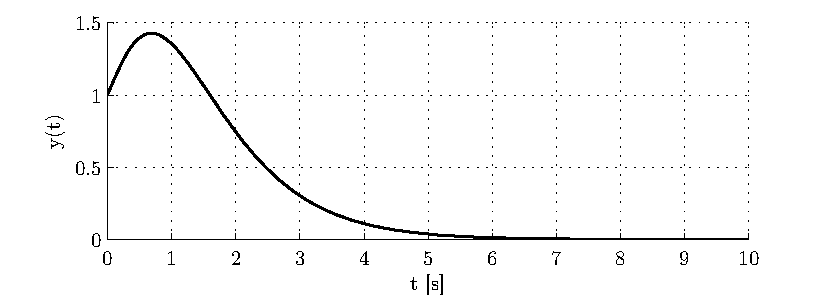
\includegraphics{Obr_Laplaceovou.pdf}
    }

	\caption{Grafické znázornenie riešenia získaného pomocou Laplaceovej transformácie}
	\label{Grafické znázornenie riešenia získaného pomocou Laplaceovej transformácie}
\end{figure}








\section{Otázky a úlohy}

\begin{enumerate}[leftmargin=0pt, labelsep=3mm, itemsep=0pt]

    \item Napíšte vzťah (rovnicu), ktorým je definovaná Laplaceova transformácia.

    \item Napíšte Laplaceov obraz derivácie časovej funkcie $\frac{\text{d}f(t)}{dt}$.

    \item Napíšte Laplaceov obraz jednotkového skoku.

    \item Napíšte Laplaceov obraz Dirackovho impulzu.

    \item Nájdite analytické riešenie diferenciálnej rovnice s využitím Laplaceovej transformácie.
    \begin{align*}
        \dot y(t) + a_0 y(t) = b_0 u(t) \qquad y(0) = y_0 \qquad a_0, b_0, y_0\in\mathbb R \qquad u(t) = 1
    \end{align*}

    \item Nájdite analytické riešenie diferenciálnej rovnice s využitím Laplaceovej transformácie.
    \begin{align*}
        \dot y(t) + a_0 y(t) = b_0 u(t) \qquad y(0) = y_0 \qquad a_0, b_0, y_0\in\mathbb R \qquad u(t) = \delta(t)
    \end{align*}

    \item Nájdite analytické riešenie diferenciálnej rovnice s využitím Laplaceovej transformácie.
    \begin{align*}
        \ddot y(t) + (a+b) \dot y(t) + ab y(t) = 0 \qquad y(0) = y_0,\ \dot y(0) = z_0  \qquad a\in\mathbb R,\ b\in\mathbb R,\ y_0\in\mathbb R,\ z_0\in\mathbb R
    \end{align*}

    \item Nájdite analytické riešenie diferenciálnej rovnice s využitím Laplaceovej transformácie.
    \begin{align*}
        \ddot y(t) +4 \dot y(t) + 3y(t) = u(t) \qquad y(0) = 3,\ \dot y(0) = -2 \qquad u(t) = 1
    \end{align*}

    {\color{Gray} \scriptsize K dispozícii je tabuľka Laplaceových obrazov:

    \begin{center}

        \smallskip

        % \newcommand{\Laplace}[1]{\ensuremath{\mathcal{L}{\left\{#1\right\}}}}
        % \newcommand{\InvLap}[1]{\ensuremath{\mathcal{L}^{-1}{\left\{#1\right\}}}}
        \begin{tabular*}{0.68\textwidth}{c @{\extracolsep{\fill}} c}
            \toprule
            $f(t)$                                  & $\Laplace{f(t)}=F(s)$ \\
            \midrule
            $\displaystyle \frac{\text{d}^n f(t)}{\text{d}t^n}$ & $s^nF(s) - s^{(n-1)} f(0) - \cdots - f^{(n-1)}(0)$   \\ \addlinespace[2mm]
            $e^{at}$ 	                            & $\dfrac{1}{s-a}$     \\ \addlinespace[2mm]
            $1$                                     & $\dfrac{1}{s}$      \\ \addlinespace[2mm]
            $\delta(t)$	                            & $1$                 \\
            \bottomrule
        \end{tabular*}

    \end{center}
    }


\end{enumerate}















\bibliography{../misc_LaTeX/Bib_MRS}{}
% \bibliographystyle{plain}
\bibliographystyle{unsrtnat}






\end{document}
